\newcommand{\E}{\mathrm{E}}

\section{Analysis of the Challenger-Solver Game}
\label{sec:challengersolver}

For two-player zero-sum games like go and chess, extensive self-play can be expected to sufficiently explore and exploit the game rules to reach superhuman intelligence given enough compute and model capacity.
For the challenger-solver game, we show that a sufficiently intelligent challenger has several dominant strategies so the solver learns nothing useful and the self-play stops progressing. We first show that the goal of the challenger is to set an optimal target solve rate, then we outline two types of dominant strategies of the challenger. The first is a truly dominant challenger but requires a powerful action space such as ours. The second is a tunnel-vision challenger that applies to other self-play settings as well such as Absolute Zero. Finally, we discuss the role of natural language and some practical mitigations that address these problems by strong grounding and limited self-play.

\subsection{The Challenger Has an Optimal Target Solve Rate}
\label{sec:optimalchallenger}
Reward \eqref{eq:reward_inject} increases toward 0, but is negative at exactly 0. While this seems to encourage the challenger to target an arbitrarily small solve rate, ``arbitrarily small" cannot be distinguished from 0 by a small group of $G=8$ samples so some margin is needed to achieve the optimum expected reward.
We show that challenger reward \eqref{eq:reward_inject} and $r(s) = s^a(1-s)^b$ both have a unique optimal target solve rate $p^* \in (0, 1)$ where $s$ is estimated by a group of $G$ trajectories, each with a target solve rate of $p$.
To pick $p$ that maximizes the expected reward, the RL algorithm draws $k \sim \operatorname{Binom}(G, p)$ samples to get the group's empirical solve rate $s = k/G$ and the challenger gets a reward $r(s)$.
So the real goal of the challenger is to maximize the expected reward
\[R(p) =\E_{k \sim \operatorname{Binom}(G, p)}[r(k/G)] = \sum_{k=0}^G \binom{G}{k} p^k (1-p)^{G-k} r(k/G),
\]
which is a degree $G$ polynomial in the target solve rate $p$. If $r(s) = s^a(1-s)^b$, then the optimal success rate is around $p^* \approx a/(a+b)$ with increasing precision for large $G$ as the binomial becomes more concentrated. If the reward says to avoid 0 or 1 more strongly like \eqref{eq:reward_inject}, then there will be an appropriate amount of conservatism to move $p$ towards the middle, especially with small $G$. While \eqref{eq:reward_inject} appears  different from the Beta reward $r(s) = s^a(1-s)^b$, they behave similarly when viewed in terms of the expected reward as a function of the target solve rate $p$ where the discontinuity of \eqref{eq:reward_inject} disappears in expected reward. \Cref{fig:expected_reward} shows that for the expected reward, \eqref{eq:reward_inject} is similar to the Beta reward with appropriate $a$ and $b$, and there is a unique maximum target solve probability $p^* \in (0, 1)$ around 0.2 for the challenger to achieve its optimal expected reward.

\begin{figure}[h!]
    \centering
    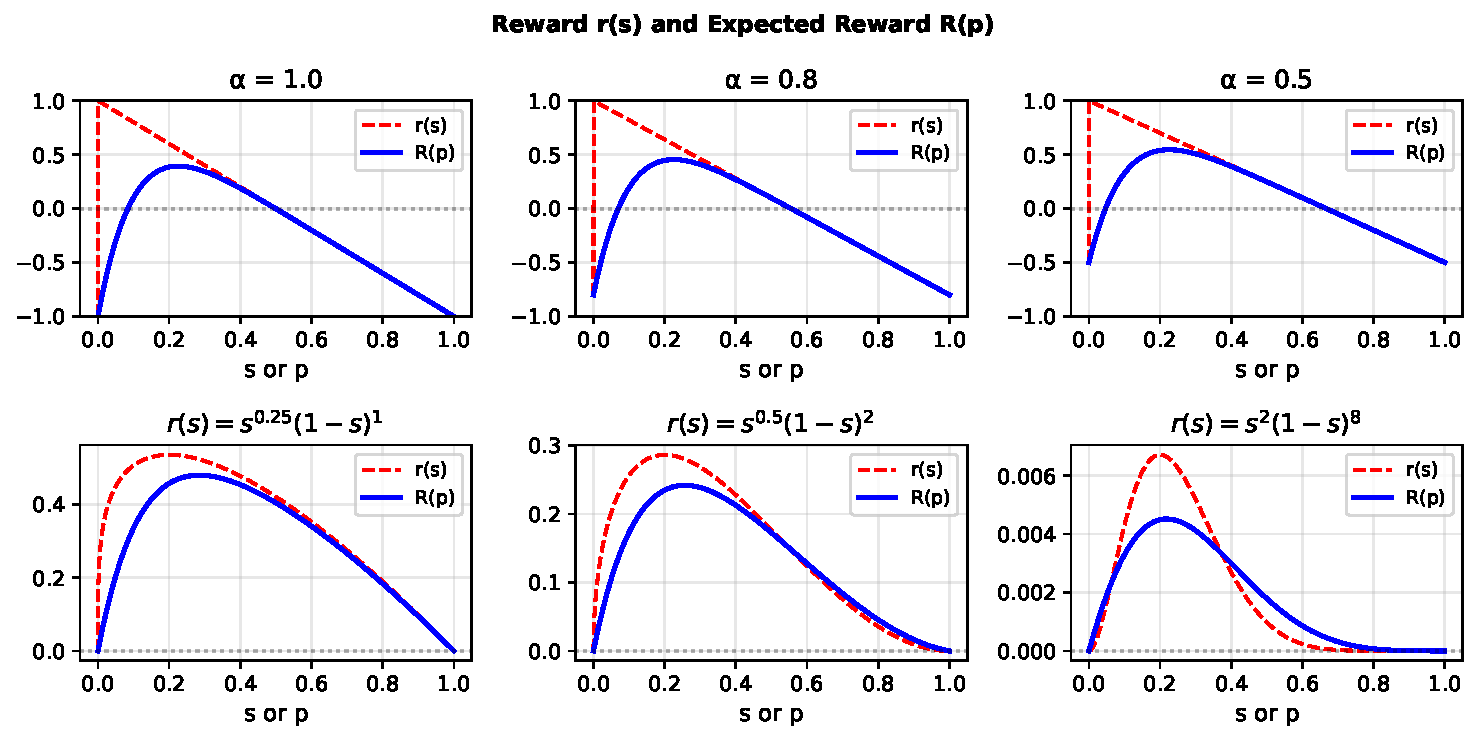
\includegraphics[width=0.85\linewidth]{plots/expected_reward_plot.pdf}
    \caption{Expected reward $R(p)$ using $G=8$ vs. the target solve rate $p$ plotted with the original reward function $r(s)$ for context. The expected reward applies a smoothing function and lessens the difference between various reward choices $r(s)$. While $\alpha$ only shifts the reward function, it can affect the relative weighting of other failure types (such as consistency or system error) so it is an appropriate single-purpose parameter.}
    \label{fig:expected_reward}
\end{figure}

\subsection{The Challenger Strategy}
\label{sec:cheatingchallenger}
While the solver achieves its sensible optimal reward by solving all the problems, the challenger can employ several strategies to achieve its own optimal reward at the cost of the solver.

\paragraph{The dominant challenger.} The challenger has a \textit{dominant strategy} if it can output a question that is solved with probability $p^*$ and achieve its own optimal reward regardless of what the solver does. This is possible when the challenger has sufficient freedom to set the problem.

The most direct way is when the challenger is allowed to modify the tests, then one such test is \textbf{fail-randomly}: $\texttt{if rand() < p: pass(); else: fail()}$. If we try to fix this by requiring determinism, we can use the code text of the solution to generate a pseudo-random number instead,
\[\texttt{if rand(seed=hash(current\_code)) < p: pass(); else: fail()}\]
where the pseudo-random function returns the same number on the same code, which works as long as the sampled solutions are different. If we require that the original code must pass, the test can have a case for the original code too $\texttt{if hash(current\_code) = hash(original\_code): pass()}$, where the original code hash is a constant, and the current code is read from the files.

Even when the test is fixed, one strategy is the following:
\begin{enumerate}
    \item Add the \textbf{fail-randomly} method (or its pseudo-random extension) to return the wrong output at random or just raise an exception.
    \item Obfuscate the whole codebase so it is impossible for the solver to find and fix the change.
\end{enumerate}
Here the solver cannot improve on the proposed problem assuming that we have good enough obfuscation so the solver cannot understand the code. The solver can make it worse but has no incentive to, so the best response for the solver is to do nothing\footnote{Thus not technically a dominant strategy, but still strong.}.
It seems hard to prevent this theoretical behavior as long as the challenger has a Turing complete action space to take actions such as these. In practice, if the challenger does not have an awareness of its own setting, it may not be able to design such optimal strategies even if it is superintelligent.

\paragraph{The tunnel-vision challenger.}
Even if the challenger has a limited actions space, the challenger can still focus its tunnel-vision on one specific parameter to control the difficulty and does not cover the diversity that we want the solver to learn. Since the solver cannot keep improving on any specific task, learning eventually stops and the challenger achieves its optimal expected reward. For example, suppose that long multiplication is challenging for the solver, the challenger can just adjust the length of the operands until it is at the desired difficulty. Even as the solver learns, it presumably cannot learn to do infinity long multiplications and thus will be stuck at a desired accuracy as the length increases and the challenger is optimal. In the software setting, the challenger can hide a particular type of bug with increasing level of obfuscation. Another method is to chain a number of medium solve rate challenges together, and the solver has to solve all of them to pass, and the challenger can adjust the chain length appropriately without covering diverse challenges outside of this arbitrary and narrow tunnel of problems.

\paragraph{Improving natural language communication with humans.}
We argue that deep self-play without human language grounding or human interaction is unpromising, at least if the goal is to communicate well with current humans.
Diplomacy \cite{bakhtin2022human} argues that when learning to cooperate with humans, \emph{self-play without human data is no longer
guaranteed to find a policy that performs well
with humans.} This is clearly demonstrated by the Ultimatum game, where the optimal play of always accept any positive offer is quite different from human behavior, which has fairness and ego built-in. Learning to solve human problems and fixing human issues where natural language plays a major role is an example of cooperating with humans.
In any particular game where communication is needed, there are many sufficient \textit{languages}, where many are more efficient than natural language because they can specialize to this setting only. While deep self-play can improve communication skills, it would not plausibly stay with and improve the quality of its human natural language even when initialized by a LLM trained on natural language. 
For some examples, \cite{kottur2017natural} shows effective communication in games needs not to be like human language or even compositional. In learning language games \cite{wang2016learning}, humans are observed to adapt to a particular grounding and stop using standard language. To draw another analogy, we note that human languages also evolve and change to become unrecognizable over a long period of time,%
\footnote{A popular introduction is \textit{The Power of Babel: A Natural History of Language}}
or even over a short amount of time in the case of software engineering writing laden with Three-Letter Acronyms (TLA) evolved from self-play by closed teams incomprehensible to anyone outside.


\paragraph{Mitigations.}
Since the challenger has a dominant strategy, we do not desire enough self-play to fully explore and exploit the implications of the game rules, unlike for 2-player zero-sum games. However, a shallower challenger can still be beneficial by taking advantage of the model's ability to  generate and explore diverse challenges and without learning to adopt its best strategy.
In particular,
\begin{enumerate}
    \item The challenger should be grounded in large and diverse real world data, such as all code repositories or documents. The goal is to skillfully pose natural and diverse challenges grounded in and inspired by real data. 
    \item Do not let the challenger diverge much from the initial instruction-based strategy and ensure that the self-play does not reach the tunnel-vision strategy. The challenger can still learn skills like passing the consistency checks and some calibration of question difficulty.
    \item Do not attempt to improve on natural language skills using self-play without continued grounding on current human natural language. Gaining technical skills and code world model knowledge from self-play is desirable and plausible.
\end{enumerate}








\section{Opposing Incentives in the Reward Design}

The solve rate $s$ in \cref{eq:reward_inject} is computed over all solver attempts (e.g., 8 attempts per bug).
Each individual solver attempt receives the binary reward $r_{\text{solve}} \in \{+1, -1\}$ based solely on whether it succeeds. Given a bug with solve rate $s$, the expected solver reward is $\mathbb{E}[r_{\text{solve}}] = s - (1-s) = 2s - 1$.
For valid bugs with ideal difficulty ($0 < s < 1$), the injection reward simplifies to $r_{\text{inject}} = 1 - (1 + \alpha) s$.
Consequently, the solver benefits from higher $s$ (easier bugs increase expected reward), while the injector benefits from lower $s$ (harder bugs increase injection reward), though bugs that are too hard ($s = 0$) are penalized to prevent unsolvable proposals. This adversarial pressure pushes the injector to propose bugs near the frontier of the solver's current capability. Note the optimal target difficulty depends on the sample size, explained in \cref{sec:challengersolver}.

\section{Experimental Details}

\paragraph{Training details.}
We implement \tech on top of the async \cwm-RL infrastructure~\cite{faircodegenteam2025cwmopenweightsllmresearch} and adopt the same RL algorithm, with some hyperparameter modifications.
We train the models on NVIDIA H100 SXM 80G GPUs, with a standard configuration of 512 GPUs for a single training run, with 64 GPUs for training and 448 GPUs for rollouts.
Inspired by ScaleRL~\cite{khatri2025artscalingreinforcementlearning} and MiniRL~\cite{qwenstablerl}, we incorporate a ``large-batch'' and ``small-policy-staleness'' hyperparameter setup.
By default, we employ a 131,072 maximum context window size for generation,
pack training sequences by a maximum of 131,072 tokens,
use a global batch size of 16M tokens, achieved through 16 gradient accumulation steps per optimizer step,
and a typical group size of 8 for acceptable rollout latency,
discard rollouts with more than 8 off-policy steps,
and train the models (including baseline RL, \tech, and all ablation runs) for 150 global steps, roughly 2.5B tokens, with 30 steps of learning rate warmup toward $3\times 10^{-6}$.


Our implementation employs the same tool-based scaffold as \cwm with minor prompt adjustments, incorporating Bash and a search-replace editor. All environment images used in our experiments are identical to those in \cwm.

\paragraph{Evaluation noise.}
While our method demonstrates consistent self-improvements across the training steps, we acknowledge the presence of evaluation noise, typically around 2\% paired standard error on \sbv. Readers can refer to Eval~Arena~\cite{evalarena} for a detailed discussion.



\section{Prompt Templates}
\subsection{Bug Injection}
\label{sec:apd:prompt_bug_injection}

\begin{promptbox}{Removal-oriented bug-injection}
    \begin{Verbatim}[breaklines=true]
You are working with a random commit from a code repository. Your goal is to introduce **complex bugs** into the codebase by removing multiple code files or code chunks and then removing tests to hide the bugs. The bugs will serve as training data for a bug-fixing AI system.

### Steps to follow

1. Understand the codebase, its functionalities, and the test suite / framework / command structure.
2. **Identify interesting test files**: find a set of test files that cover significant functionality in the codebase, making sure they involve at least {min_passing_tests} tests and test over {min_changed_files} code files.
3. **Set up the test command**: Create a test command that runs your selected tests. Make sure your test command can output the detailed test results, including which tests passed or failed (e.g., `pytest -rA`); ensure that the test execution takes less than 90 seconds. Dump the test command in a bash script (e.g., `test_script.sh`, which may involve additional setups like environment variables) for later use.
4. Trigger the test command, **directing the output to a log file** (e.g., using `bash test_script.sh > test_output_existing_tests.log 2>&1`) because the test output can be very long. View the log file (e.g., using `head` or `tail`) to verify the results.
5. If not all tests pass, it may be due to flakiness or environment issues; just exclude them from the test command or find another set until all selected tests pass (still needs to satisfy the minimum passing tests requirement: >= {min_passing_tests}).
6. Write a generic parser script in Python that can parse any test log file output by your test command. The test script should read from stdin the test log output and writes to stdout a JSON summary mapping each executed test case to either "passed" or "failed". Verify that your parser works. Example usage and output:

```bash
$ cat test_output_existing_tests.log | python3 parse_test_output.py > test_output_existing_tests.json
$ head -n 20 test_output_existing_tests.json # avoid showing too many lines
{{
    "test_module1.py::TestClass::test_method1": "passed",
    "test_module2.py::test_function2": "passed",
    ...
```

7. **Remove relevant code files or chunks**: Based on your exploration in step 2, introduce bugs by removing hunks or directly deleting all content from at least {min_changed_files} code files.
8. Run the original test command again and make sure some tests fail, meaning the removal breaks some functionality. Don't introduce additional syntax errors that make all tests fail. Still, redirect the output to a log file (e.g., `bash test_script.sh > test_output_bug_code.log 2>&1`) to view the results. Also, verify that your parser script can correctly parse the test results log and summarize which tests passed or failed. For example:

```bash
$ cat test_output_bug_code.log | python3 parse_test_output.py > test_output_bug_code.json
$ cat test_output_bug_code.json | grep "failed"
...
```

9. **Create the bug patch (code files only)**: Construct a bug patch for your changes using `git diff`. For example, `git diff > bug_patch.diff`. Because `git diff` won't apply to files in the index / untracked files, make sure you correctly create the bug patch (either stage all the changes and then use `git diff --cached`, or use `git diff` for tracked files). Review that the bug patch captures the intended reversions and compatibility fixes. **Verify that the patch ONLY contains changes to code files, NOT test files.**
10. **Remove/weaken tests (ONLY test files can be modified)**: Now and only now, you can modify test files. Delete entire test functions, files or remove / weaken some of the test cases that would catch your bug, creating a "test gap" where some bugs can hide. **CRITICAL: DO NOT comment out the original tests as this leaves obvious hints; instead, simply delete them or weaken assertions.**
11. **Create the test weakening patch (test files only)**: Create a test weakening patch using `git diff` but only on the test files you modified. **Verify that this patch ONLY contains changes to test files, NOT code files.**

### IMPORTANT REQUIREMENTS

1. There MUST be AT LEAST {min_passing_tests} tests passing before the bug is introduced.
2. The bug patch MUST modify AT LEAST {min_changed_files} code files (NOT test files). Modification includes adding, removing, or editing files.
3. You MUST NOT leave any hints that reveals your bug injection intention. DO NOT leave comments like "introduce bug here" in your patches. DO NOT leave the original correct code in comments.
4. VERY IMPORTANT: ALL modified code files in the bug patch MUST be covered by some test(s) in your test command. There must be NO orphan code files that are modified but not exercised by any of the selected tests.

### Required files to submit

1. test_files.txt: A text file listing all the test files you selected in step 2 to validate (1) the original code correctness and (2) the bug exposure after code removal (one unique **relative** file path per line).
2. test_script.sh: A bash script specifying how to run the tests
3. parse_test_output.py: A Python script that parses the test output log and summarizes the detailed results (test_id -> passed / failed) in JSON format.
4. bug_patch.diff: A git diff patch that introduces the bug into the code.
5. test_patch.diff: A git diff patch that removes/weakens tests to hide the bug.

### Submission format

<tool: submit>
test_files.txt
test_script.sh
parse_test_output.py
bug_patch.diff
test_patch.diff
</tool>

I've uploaded the corresponding code repository at {repo_root} and installed all the necessary dependencies. Now, the bash session has started, with the current working directory set to the repo root. 
\end{Verbatim}
\end{promptbox}

\begin{promptbox}{History-aware bug-injection}
\begin{Verbatim}[breaklines=true]
You are working with a random commit from a code repository. Your goal is to introduce **realistic bugs** into the codebase by selectively reverting code changes from git history and applying minimal compatibility fixes to ensure the code remains runnable. The bugs will serve as training data for a bug-fixing AI system.

The bug introduction process involves two key steps:
1. **Selectively revert code changes from history**: Use git history to identify and revert specific bug fixes or improvements. You can revert entire files to historical versions, cherry-pick specific line ranges from previous commits, or combine reversions from multiple commits across multiple files. This gives you fine-grained control over bug introduction.
2. **Apply minimal compatibility fixes**: Make only the necessary adjustments to resolve trivial issues (e.g., import errors, renamed functions, API changes) so the code runs without syntax errors, while preserving the historical bugs.

### Steps to follow

1. Understand the codebase, its functionalities, and the test suite / framework / command structure.
2. **Browse git history to identify revertible changes**: Use `git log`, `git log --oneline`, `git show`, `git diff`, `git log -p`, and `git log -L <start>,<end>:<file>` (for line-range history) to explore the repository's history. Look for commits that introduced bug fixes, refactorings, or improvements to core functionality that you can revert. Focus on:
   - Bug fix commits (search for keywords like "fix", "bug", "issue", "crash", "error" in commit messages)
   - Feature enhancements or optimizations that can be reverted
   - Edge case handling that can be removed

   Identify interesting changes across code files (NOT test files) that you might want to revert. These can be:
   - Entire file restorations to historical versions
   - Specific function/method changes from particular commits
   - Line-range reversions using `git show <commit>:<file>` and manual editing
   - Combinations of multiple partial reversions across different files

   Take detailed notes on which commits, files, and line ranges contain revertible changes.
3. **Identify related tests**: Based on the code changes you've identified in step 2, find the corresponding test files that exercise those code paths. You can use `git log` on test files, search for imports/references, or run tests to see which ones are related. Select a test suite that includes at least {min_passing_tests} tests related to your target code files. The tests can also be indirectly related if you cannot find enough direct tests.
4. **Set up the test command**: Create a test command that runs your selected tests. Make sure your test command can output the detailed test results, including which tests passed or failed (e.g., `pytest -rA`); ensure that the test execution takes less than 90 seconds. Dump the test command in a bash script (e.g., `test_script.sh`, which may involve additional setups like environment variables) for later use.
5. Trigger the test command, **directing the output to a log file** (e.g., using `bash test_script.sh > test_output_existing_tests.log 2>&1`) because the test output can be very long. View the log file (e.g., using `head` or `tail`) to verify the results.
6. If not all tests pass, it may be due to flakiness or environment issues; just exclude them from the test command or find another set until all selected tests pass (still needs to satisfy the minimum passing tests requirement: >= {min_passing_tests}).
7. Write a generic parser script in Python that can parse any test log file output by your test command. The test script should read from stdin the test log output and writes to stdout a JSON summary mapping each executed test case to either "passed" or "failed". Verify that your parser works. Example usage and output:

```bash
$ cat test_output_existing_tests.log | python3 parse_test_output.py > test_output_existing_tests.json
$ head -n 20 test_output_existing_tests.json # avoid showing too many lines
{{
    "test_module1.py::TestClass::test_method1": "passed",
    "test_module2.py::test_function2": "passed",
    ...
```

8. **Selectively revert code changes (NO TEST FILES)**: Based on your exploration in step 2, introduce bugs by reverting changes to at least {min_changed_files} code files (NOT test files). You have multiple strategies available:

   **Strategy A: Full file restoration**
   - Restore entire files to historical versions using `git show <commit>:path/to/file > path/to/file` or `git restore --source=<commit> --worktree -- path/to/file`

   **Strategy B: Cherry-pick specific changes**
   - Use `git show <commit>` to view specific bug fixes
   - Use `git show <commit>:<file>` to see how specific files looked at that commit
   - Use `git log -L <start>,<end>:<file>` to see the history of specific line ranges
   - Manually revert just the relevant portions of those fixes by editing files

   **Strategy C: Combine multiple reversions**
   - Revert different changes from different commits across multiple files
   - Create complex multi-file bugs by reverting related changes in dependent components
   - Mix full file restorations with partial cherry-picked reversions

   **Examples of history-viewing commands:**
   ```bash
   # View a specific commit's changes
   git show <commit_hash>

   # View how a file looked at a specific commit
   git show <commit_hash>:path/to/file

   # View history of specific line range in a file (at most recent <N> commits)
   git log -L 10,20:path/to/file -n <N>

   # Restore entire file to historical version
   git show <commit_hash>:path/to/file > path/to/file

   # View diff between two commits for a file
   git diff <old_commit>..<new_commit> -- path/to/file
   ```

   Choose the strategy or combination of strategies that creates the most realistic bugs. The key is to revert actual bug fixes or improvements that were previously made, not to introduce arbitrary syntax errors.

   **CRITICAL: You MUST NOT modify or restore any test files in this step - only code files!**
9. **Apply minimal compatibility fixes (ONLY to code files)**: After reverting code changes, apply minimal compatibility fixes to resolve only the trivial issues that prevent the code from running (e.g., import errors, renamed functions, API changes). Make only the necessary adjustments to ensure tests can execute without syntax errors, while preserving the reverted bugs. **Do NOT modify any test files in this step.** Then run the original test command again and make sure some tests fail, meaning the reverted bugs would be caught by the original tests. Don't introduce additional syntax errors that make all tests fail. Still, redirect the output to a log file (e.g., `bash test_script.sh > test_output_buggy_code.log 2>&1`) to view the results. Also, verify that your parser script can correctly parse the test results log and summarize which tests passed or failed. For example:

```bash
$ cat test_output_buggy_code.log | python3 parse_test_output.py > test_output_buggy_code.json
$ cat test_output_buggy_code.json | grep "failed"
...
```

10. **Create the bug patch (code files only)**: Construct a bug patch for your changes (reverted changes + minimal compatibility fixes) using `git diff`. For example, `git diff > bug_patch.diff`. Because `git diff` won't apply to files in the index / untracked files, make sure you correctly create the bug patch (either stage all the changes and then use `git diff --cached`, or use `git diff` for tracked files). Review that the bug patch captures the intended reversions and compatibility fixes. **Verify that the patch ONLY contains changes to code files, NOT test files.**
11. **Weaken tests (ONLY test files can be modified)**: Now and only now, you can modify test files. Remove or weaken some of the tests that would catch your bug, creating a "test gap" where some bugs can hide. You can remove test cases, weaken assertions, remove edge case coverage that exposes the bug, or simply reverting the test to a historical version. You don't need to hide ALL test failures; it's acceptable if some tests still fail after weakening. **CRITICAL: In this step, you MUST ONLY modify test files. Do NOT modify any code files.** Once done, run the test command again and verify that fewer tests fail compared to step 9. Still redirect the output to a log file (e.g., `bash test_script.sh > test_output_weakened_tests.log 2>&1`) to view the results and verify the parser script works as expected. **CRITICAL: DO NOT comment out failing tests as this leaves obvious hints; instead, simply delete them or weaken assertions.**
12. **Create the test weakening patch (test files only)**: Create a test weakening patch using `git diff` but only on the test files you modified. **Verify that this patch ONLY contains changes to test files, NOT code files.**

### IMPORTANT REQUIREMENTS

1. There MUST be AT LEAST {min_passing_tests} tests passing before the bug is introduced.
2. The bug patch MUST modify AT LEAST {min_changed_files} code files (NOT test files). Modification includes adding, removing, or editing files.
3. After introducing the bug, AT LEAST {min_num_tests_to_break} tests MUST fail.
4. You MUST NOT leave any hints that reveals your bug injection intention. DO NOT leave comments like "introduce bug here" in your patches. DO NOT leave the original correct code in comments.
5. VERY IMPORTANT: ALL modified code files in the bug patch MUST be covered by some test(s) in your test command. There must be NO orphan code files that are modified but not exercised by any of the selected tests.
6. The bug MUST be realistic, something that can naturally occur in a code project. DO NOT introduce syntax errors or undefined variables that make all tests fail.

### Required files to submit

1. test_files.txt: A text file listing all the test files you selected in step 2.
2. test_script.sh: A bash script specifying how to run the tests
3. parse_test_output.py: A Python script that parses the test output log and summarizes the detailed results (test_id -> passed / failed) in JSON format.
4. bug_patch.diff: A git diff patch that introduces the bug into the code.
5. test_patch.diff: A git diff patch that removes/weakens tests to hide the bug.

### Submission format

<tool: submit>
test_files.txt
test_script.sh
parse_test_output.py
bug_patch.diff
test_patch.diff
</tool>

I've uploaded the corresponding code repository at {repo_root} and installed all the necessary dependencies. Now, the bash session has started, with the current working directory set to the repo root.
\end{Verbatim}
\end{promptbox}

\begin{promptbox}{Direct bug-injection}
\begin{Verbatim}[breaklines=true]
You are working with a random commit from a code repository. Your goal is to introduce bugs into the codebase.

### Steps to follow

1. Understand the codebase, its functionalities, and the test suite / framework / command structure.
2. **Identify interesting test files**: find a set of test files that cover significant functionality in the codebase, making sure they involve at least {min_passing_tests} tests and test over {min_changed_files} code files.
3. **Set up the test command**: Create a test command that runs your selected tests. Make sure your test command can output the detailed test results, including which tests passed or failed (e.g., `pytest -rA`); ensure that the test execution takes less than 90 seconds. Dump the test command in a bash script (e.g., `test_script.sh`, which may involve additional setups like environment variables) for later use.
4. Trigger the test command, **directing the output to a log file** (e.g., using `bash test_script.sh > test_output_existing_tests.log 2>&1`) because the test output can be very long. View the log file (e.g., using `head` or `tail`) to verify the results.
5. If not all tests pass, it may be due to flakiness or environment issues; just exclude them from the test command or find another set until all selected tests pass (still needs to satisfy the minimum passing tests requirement: >= {min_passing_tests}).
6. Write a generic parser script in Python that can parse any test log file output by your test command. The test script should read from stdin the test log output and writes to stdout a JSON summary mapping each executed test case to either "passed" or "failed". Verify that your parser works. Example usage and output:

```bash
$ cat test_output_existing_tests.log | python3 parse_test_output.py > test_output_existing_tests.json
$ head -n 20 test_output_existing_tests.json # avoid showing too many lines
{{
    "test_module1.py::TestClass::test_method1": "passed",
    "test_module2.py::test_function2": "passed",
    ...
```

7. **Introduce bugs**: Based on your exploration in step 2, introduce bugs to at least {min_changed_files} code files.
8. Run the original test command again and make sure some tests fail, meaning the bug breaks some functionality. Don't introduce trivial syntax errors that make all tests fail. Still, redirect the output to a log file (e.g., `bash test_script.sh > test_output_bug_code.log 2>&1`) to view the results. Also, verify that your parser script can correctly parse the test results log and summarize which tests passed or failed. For example:

```bash
$ cat test_output_bug_code.log | python3 parse_test_output.py > test_output_bug_code.json
$ cat test_output_bug_code.json | grep "failed"
...
```

9. **Create the bug patch (code files only)**: Construct a bug patch for your changes using `git diff`. For example, `git diff > bug_patch.diff`. Because `git diff` won't apply to files in the index / untracked files, make sure you correctly create the bug patch (either stage all the changes and then use `git diff --cached`, or use `git diff` for tracked files). Review that the bug patch captures the intended reversions and compatibility fixes. **Verify that the patch ONLY contains changes to code files, NOT test files.**
10. **Weaken tests (ONLY test files can be modified)**: Now and only now, you can modify test files. Weaken / remove some of the test cases that would catch your bug, creating a "test gap" where some bugs can hide. **CRITICAL: DO NOT comment out the original tests as this leaves obvious hints; instead, simply delete them or weaken assertions.**
11. **Create the test weakening patch (test files only)**: Create a test weakening patch using `git diff` but only on the test files you modified. **Verify that this patch ONLY contains changes to test files, NOT code files.**

### IMPORTANT REQUIREMENTS

1. There MUST be AT LEAST {min_passing_tests} tests passing before the bug is introduced.
2. The bug patch MUST modify AT LEAST {min_changed_files} code files (NOT test files).
3. After introducing the bug, AT LEAST {min_num_tests_to_break} tests MUST fail.
4. You MUST NOT leave any hints that reveals your bug injection intention. DO NOT leave comments like "introduce bug here" in your patches. DO NOT leave the original correct code in comments.
5. VERY IMPORTANT: ALL modified code files in the bug patch MUST be covered by some test(s) in your test command. There must be NO orphan code files that are modified but not exercised by any of the selected tests.

### Required files to submit

1. test_files.txt: A text file listing all the test files you selected in step 2
2. test_script.sh: A bash script specifying how to run the tests
3. parse_test_output.py: A Python script that parses the test output log and summarizes the detailed results (test_id -> passed / failed) in JSON format.
4. bug_patch.diff: A git diff patch that introduces the bug into the code.
5. test_patch.diff: A git diff patch that removes/weakens tests to hide the bug.

### Submission format

<tool: submit>
test_files.txt
test_script.sh
parse_test_output.py
bug_patch.diff
test_patch.diff
</tool>

I've uploaded the corresponding code repository at {repo_root} and installed all the necessary dependencies. Now, the bash session has started, with the current working directory set to the repo root.
\end{Verbatim}
\end{promptbox}


\subsection{Bug Solving}
\label{sec:apd:prompt_bug_solving}

For bug-solving with our solver agent, we instantiate the issue description with the following fixed prompt template:

\begin{promptbox}{Fixed-template issue description specified by the oracle test patch}
    \begin{Verbatim}[breaklines=true]
I am improving the test suite of the project with the following changes, but the current code does not pass the tests. Please fix the code. If any existing tests relevant to the functionality being changed are failing, please make sure your patch passes those tests as well.

```diff
{oracle_test_patch}
```
\end{Verbatim}
\end{promptbox}

We then use the following prompt for general issue solving, including both the real issues from evaluation and the fixed-template issues above:

\begin{promptbox}{Prompt template for bug-solving}
\begin{Verbatim}[breaklines=true]
Solve the following issue by implementing the necessary code changes and submitting a patch file:

<issue_description>
{issue}
</issue_description>

The [result] argument of <tool: submit> should be the path to a patch file that resolves the issue. This file must be accessible from the current working directory and should contain the end-to-end code changes in git diff format. You can refine and submit your patch multiple times as needed to ensure correctness.

Once you've submitted at least once, provide a brief summary.

Again, if you have enough budget, you should try to fully utilize it by doing more testing, checking edge cases, or even considering alternative solutions. This will help you gain more confidence in your submission. DO AS MUCH TESTING AS POSSIBLE WHENEVER YOU HAVE BUDGET. The testing involves developing new tests, confirming no existing tests are broken, and checking edge cases. Only submit when all the relevant tests pass!!

I've uploaded the corresponding code repository at {repo_root} and installed all the necessary dependencies. Now, the bash session has started, with the current working directory set to the repo root.
\end{Verbatim}
\end{promptbox}


\section{Discussion}

\label{section:discussion}

\subsection{Theoretical Analysis}

With a focus on the challenger (bug-injector), we analyze the behavior of reward designs such as \cref{eq:reward_inject} and the theoretical optimal play of the challenger-solver game
in \cref{sec:challengersolver}. We show that the challenger has several dominant strategies that can stop self-play from progressing and then discuss practical mitigations that may address these problems, some of which were adopted by this work. Our analysis help clarify what we can expect in such self-play and what must be avoided. 

\subsection{Limitations}

While Self-play SWE-RL demonstrates promising results toward training superintelligent software agents, it is still an early step and several limitations warrant discussion:
\begin{itemize}
\item \textbf{No hidden oracles}: Providing the complete oracle (i.e. the tests) in the task specification prompt may enable agents to develop reward-hacking behaviors (e.g., overfitting the specific set of tests) rather than genuine bug-fixing capabilities. Although this is not observed in this paper, future iterations should explore enriching the bug artifact with public and private test splits.
\item \textbf{Unit tests for verification}: The current framework exclusively uses unit tests as the verification oracle, which represents only a subset of real-world software engineering activities. A higher-level abstraction, such as a goal, emphasized by CodeClash~\cite{yang2025codeclashbenchmarkinggoalorientedsoftware}, may serve as a more scalable way to verify software correctness.
\item \textbf{Lack of model variants and role separation:} Our experiments use a single model configuration for both roles. Future work should explore larger Mixture-of-Experts (MoE) models to understand how capacity and architecture affect self-play learning, and consider separate policies for each role.
\end{itemize}

\subsection{Unsuccessful Attempts}
We share our setbacks here for insight, but this does not imply they cannot work in the future:
\begin{itemize}
\item \textbf{Synthesizing natural language issues in self-play}: Our approach focuses on formal test specifications instead of natural language issues. While this design minimizes data assumptions and proves effective for learning, our initial attempts failed to reliably generate high-quality and unambiguous issue descriptions. The generated issues tend to copy test patches, are logically incoherent, and collapse to identical patterns. We attribute this to limited natural language capabilities of our 32B base model (\cwm) and the opaque reward signals that fail to promote quality or diversity.
\item{\bfseries Repository-specialized training}. Real-world development often involves sustained work within specific codebases where deep contextual knowledge provides significant advantages.
We explored training repository-specialized agents by performing \tech on just 23 repo images from \sbv and \sbp, preventing leakage by selecting commits prior to any evaluation instances. However, this did not outperform training on more non-overlapping repos, likely because 23 repos provide insufficient diversity in problem-solving patterns.
\item \textbf{Stable training at scale}: Despite following \cite{khatri2025artscalingreinforcementlearning,qwenstablerl}, we still observed training instability that prevents \tech from further scaling, manifesting as gibberish outputs.
This instability may stem from a combination of suboptimal hyperparameter settings, intrinsic challenges of long-horizon rollouts, model pretraining dynamics, and fundamental properties of self-play learning.
Addressing this instability is critical to understanding how self-play scales and to unlocking its full potential.
\end{itemize}

\subsection{Future Work}
Besides addressing the aforementioned limitations, our work opens several promising research directions for advancing self-play learning and superintelligence in software engineering agents:
\begin{itemize}
\item{\bfseries Distribution control with seeding:}
The current approach lacks explicit control over bug injection locations, which can lead to duplicate bugs or distribution bias when sampling multiple times from the same repository. To improve diversity, future work could adopt seeding techniques from Magicoder~\cite{magicoder}, providing the bug-injection agent with contextual information such as target code snippets or specific files to guide the generation process toward diversity. 

\item{\bfseries Synthesizing complex multi-step software tasks:} While our approach handles repository-level bug fixing, many real-world tasks require complex, multi-step workflows, such as major version migrations or building new software stacks from scratch. Our concept of higher-order bugs is a first step, introducing layered dependencies between bug injection and repair.
Enabling such tasks will require new scaffolding designs, such as multi-context rollouts spanning interdependent sessions and automated context compaction~\cite{anthropic_context_editing_compaction,openai2025gpt52codex}.

\item{\bfseries Efficient training paradigms for long-horizon software agents:} Real-world software projects, such as building a production-grade RL codebase, pose unique challenges for agent training: they span months of iterative development, involve thousands of interdependent decisions, and cannot be fully validated by unit tests alone.
Current outcome-based RL is inefficient for such tasks because sparse terminal rewards provide little signal when most trajectories fail, making credit assignment across thousands of steps intractable.
Addressing this requires new paradigms that exploit the asymmetry between generation and verification~\cite{wei2025asymmetry} for self-verification while delivering dense and structured feedback beyond scalar rewards.
\end{itemize}
